\chapter{SYSTEM DESIGN}

 \section{Use Case Model}
\begin{figure}[H]
    \centering
     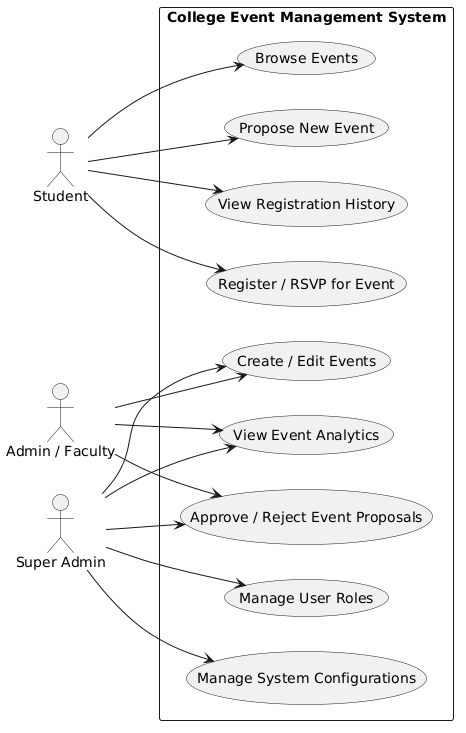
\includegraphics[width=1\textwidth,height=1\textwidth]{usecase.png}  
    \caption{Use Case Diagram - College Event Management System}
    \label{fig:Use_case}
\end{figure}
\textbf{Diagram Explanation:}\\
The Use Case diagram illustrates the overarching interactions between the system's primary actors (Super Admin, Admin/Faculty, and Student) and the application itself. 
\begin{itemize}
    \item \textbf{Student:} Interacts with the system to browse events, register/RSVP for events, view their personal registration history, and propose new events.
    \item \textbf{Admin/Faculty:} Manages the core event ecosystem. They can create new events, edit details, approve/reject student proposals, and view analytical data regarding event participation.
    \item \textbf{Super Admin:} Inherits all Admin capabilities while possessing system-wide override privileges for overarching data management.
\end{itemize}
These use cases are secured by the authentication module, ensuring actors can only perform actions permitted by their Role-Based Access Control (RBAC) level.

 \section{Activity Diagrams}
 
 \subsection{User Authentication and Routing}
\begin{figure}[H]
    \centering
     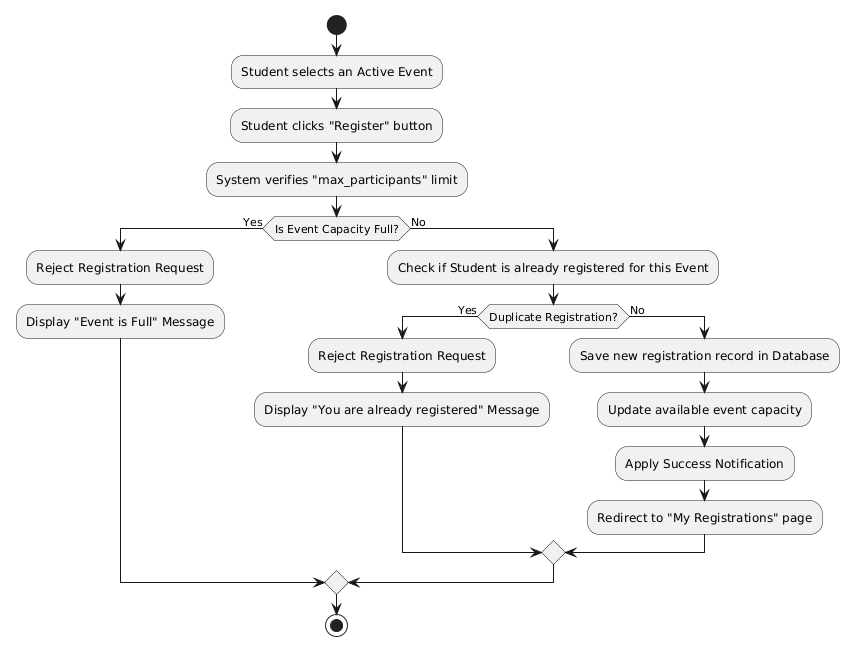
\includegraphics[width=1\textwidth,height=0.6\textwidth]{activitydiagram2.png}
    \caption{Activity Diagram - User Authentication Flow}
    \label{fig:auth_activity}
\end{figure}
\textbf{Diagram Explanation:}\\
This activity diagram represents the login and routing flow. A user enters their credentials (email and password) on the login page. The system validates the credentials against the database securely using Laravel's authentication system. If the credentials are valid, the system checks the user's assigned role. Based on the role (Student, Admin, or Super Admin), the application routes the user to their designated dashboard. If the credentials are invalid, the user is redirected back to the login page with an error message.

\subsection{Event Registration Flow}
\begin{figure}[H]
    \centering
     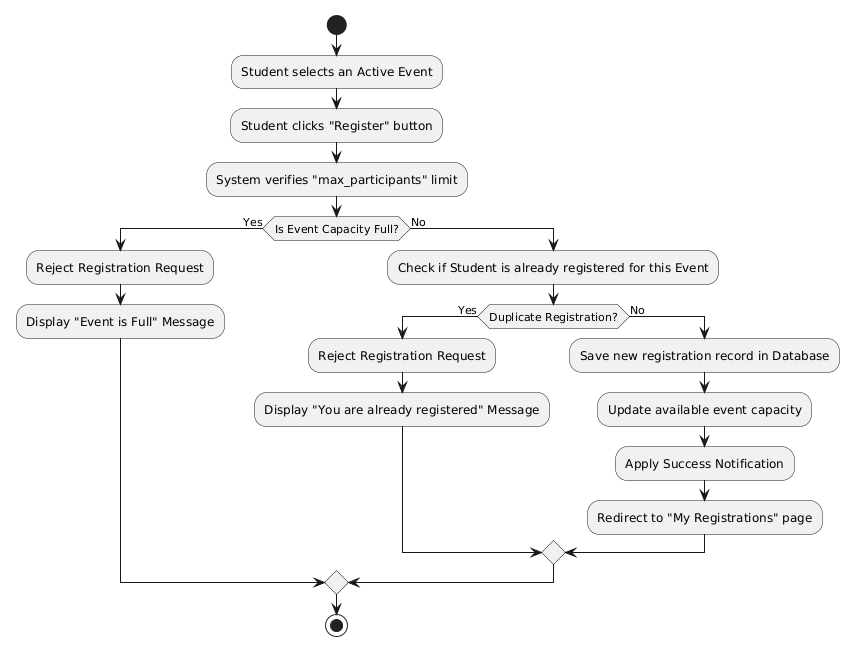
\includegraphics[width=1\textwidth]{eventdiagram.png}
    \caption{Activity Diagram - Event Registration}
    \label{fig:reg_activity}
\end{figure}
\textbf{Diagram Explanation:}\\
This diagram represents the core logic when a student attempts to register for an event. The student selects an active event and clicks "Register." The backend controller first verifying if the event has reached its \texttt{max\_participants} limit. If full, the system rejects the request. Next, it checks if the student has already registered for this specific event to prevent duplicates. If both checks pass, a new registration record is saved in the database, the available capacity is reduced, and a success notification is returned to the user.

\subsection{Sequence Diagram - Event Registration}
\begin{figure}[H]
    \centering
     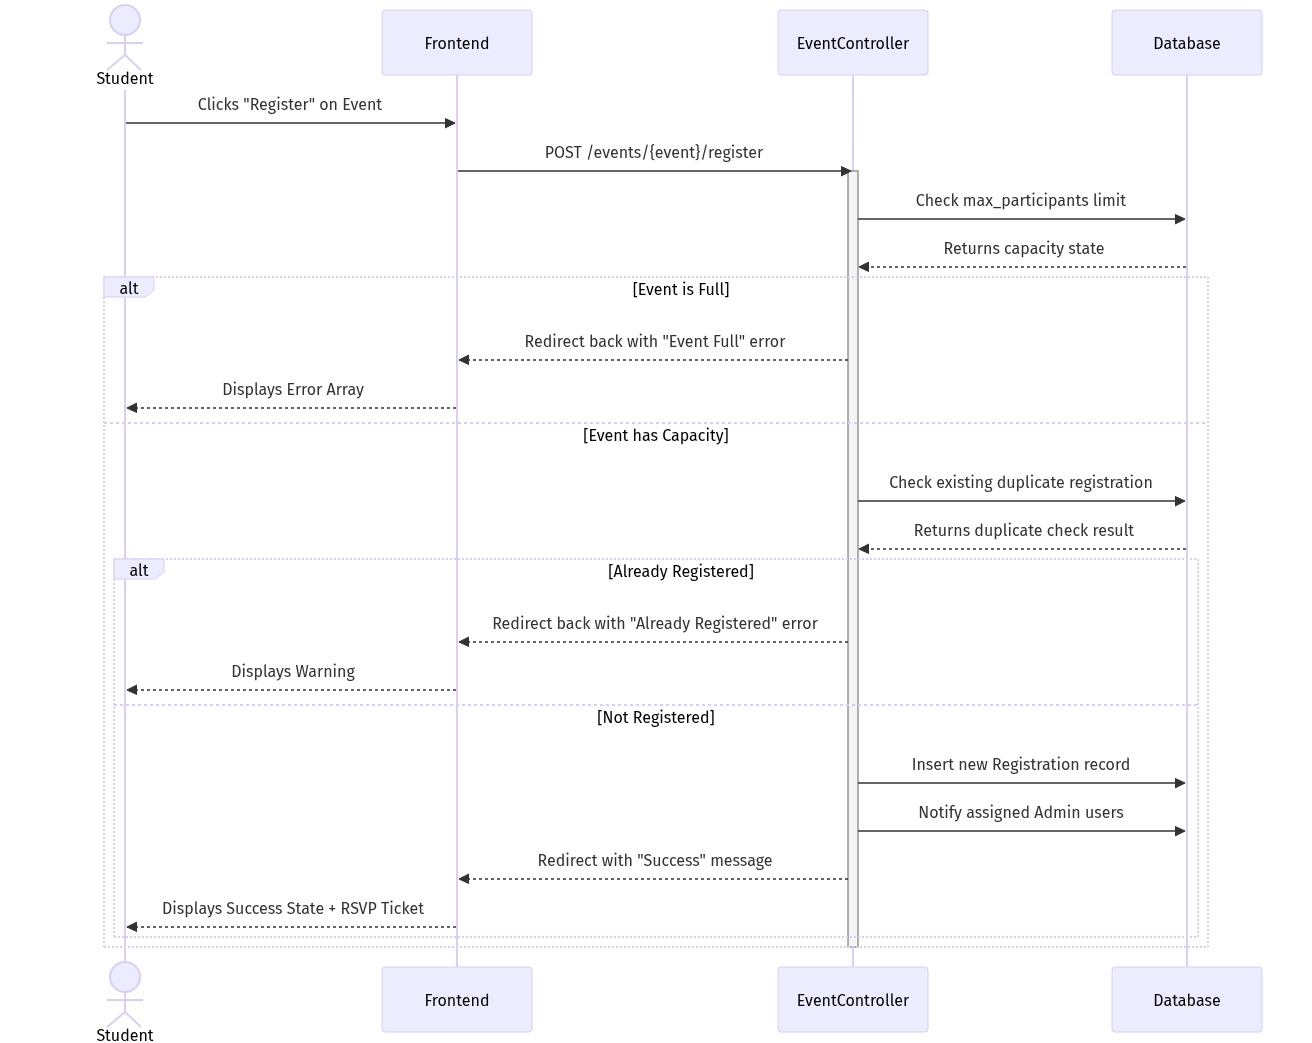
\includegraphics[width=1\textwidth]{sequencediagram.png}
    \caption{Sequence Diagram - Student Registration Flow}
    \label{fig:seq_diagram}
\end{figure}
\textbf{Diagram Explanation:}\\
The Sequence Diagram models the chronological interactions between the student, the frontend view, the EventController, and the MySQL Database during registration. It illustrates the synchronous message passing: requesting to register, validating business rules (capacity and duplication), and committing the transaction to the database, followed by returning the confirmation view.

 \section{Project Design}
 System design is the process of defining the architecture, modules, interfaces, and data for a system to satisfy specified requirements. It involves creating a robust structural foundation that ensures the application is scalable, secure, maintainable, and provides a seamless user experience.\\\\
 In the College Event Management System, the design focuses on implementing a strict Model-View-Controller (MVC) architecture using the Laravel framework. The system is designed to handle multiple user roles gracefully securely managing data flows between the backend MySQL database and the frontend interfaces. The design balances advanced administrative capabilities with a highly intuitive and accessible student-facing portal, ensuring campus events are managed efficiently without administrative bottleneck.

 \subsection{UI Design}
\textbf{(Insert screenshots and descriptions of your project's UI interfaces here, such as the Admin Dashboard, Student Portal, Event Listing Page, and Login Screen.)}
\\\\
The user interface is engineered utilizing Tailwind CSS, focusing on a clean, modern, and professional aesthetic suitable for an educational institution. The UI employs responsive design principles, ensuring dashboards and data tables render perfectly on mobile devices, tablets, and desktop monitors. Micro-interactions like button hover states, smooth transitions, and intuitive modal popups are utilized heavily to provide immediate feedback to user actions, minimizing confusion and maximizing engagement.

\subsection{System Architecture Design}
\medskip
The architecture of the College Event Management System is carefully crafted to ensure secure and efficient data processing. The system operates on a client-server model. The client-side (frontend) is rendered via Laravel Blade templates enhanced with Tailwind CSS and minimal JavaScript for dynamic UI components. \\\\
\noindent
On the server-side, Laravel acts as the robust engine handling HTTP requests, middleware filtering, and business logic execution. Middleware acts as a critical security layer; before a request reaches a controller, the middleware intercepts it to verify the user's authentication status and RBAC permissions. For example, if a student attempts to access an event-creation route, the middleware immediately blocks the request and redirects them.\\\\
\noindent
By utilizing Laravel's service container and Eloquent ORM, the application abstracts complex SQL queries into readable, object-oriented PHP code, mitigating risks like SQL injection while maintaining high performance during data retrieval.
\\\\

\subsection{Database and Schema Design}
The database serves as the single source of truth for the application, designed relationally to ensure data integrity and minimize redundancy. Instead of flat files, the system uses a robust MySQL/MariaDB database structured through Laravel Migrations. The schema is normalized and revolves around several core entities: Users, Events, Registrations, and Categories.\\\\
\textbf{Relational Structure:}\\
The database utilizes foreign keys to link data relationally. For example, the \texttt{events} table contains a \texttt{user\_id} referencing the Admin who created it. The \texttt{registrations} table acts as a pivot, linking a \texttt{student\_id} to an \texttt{event\_id}. This relational design allows the system to easily query complex datasets, such as "fetch all events categorized as 'Sports' that a specific student is registered for."
\\\\
In the application, when an administrator creates an event, the system inserts a record containing the title, description, date, location, category, and maximum capacity into the database. When a student registers, this data is cross-referenced instantaneously. This structured, relational approach ensures the system can effortlessly scale to handle thousands of users and event records simultaneously without performance degradation.

\begin{figure}[H]
    \centering
    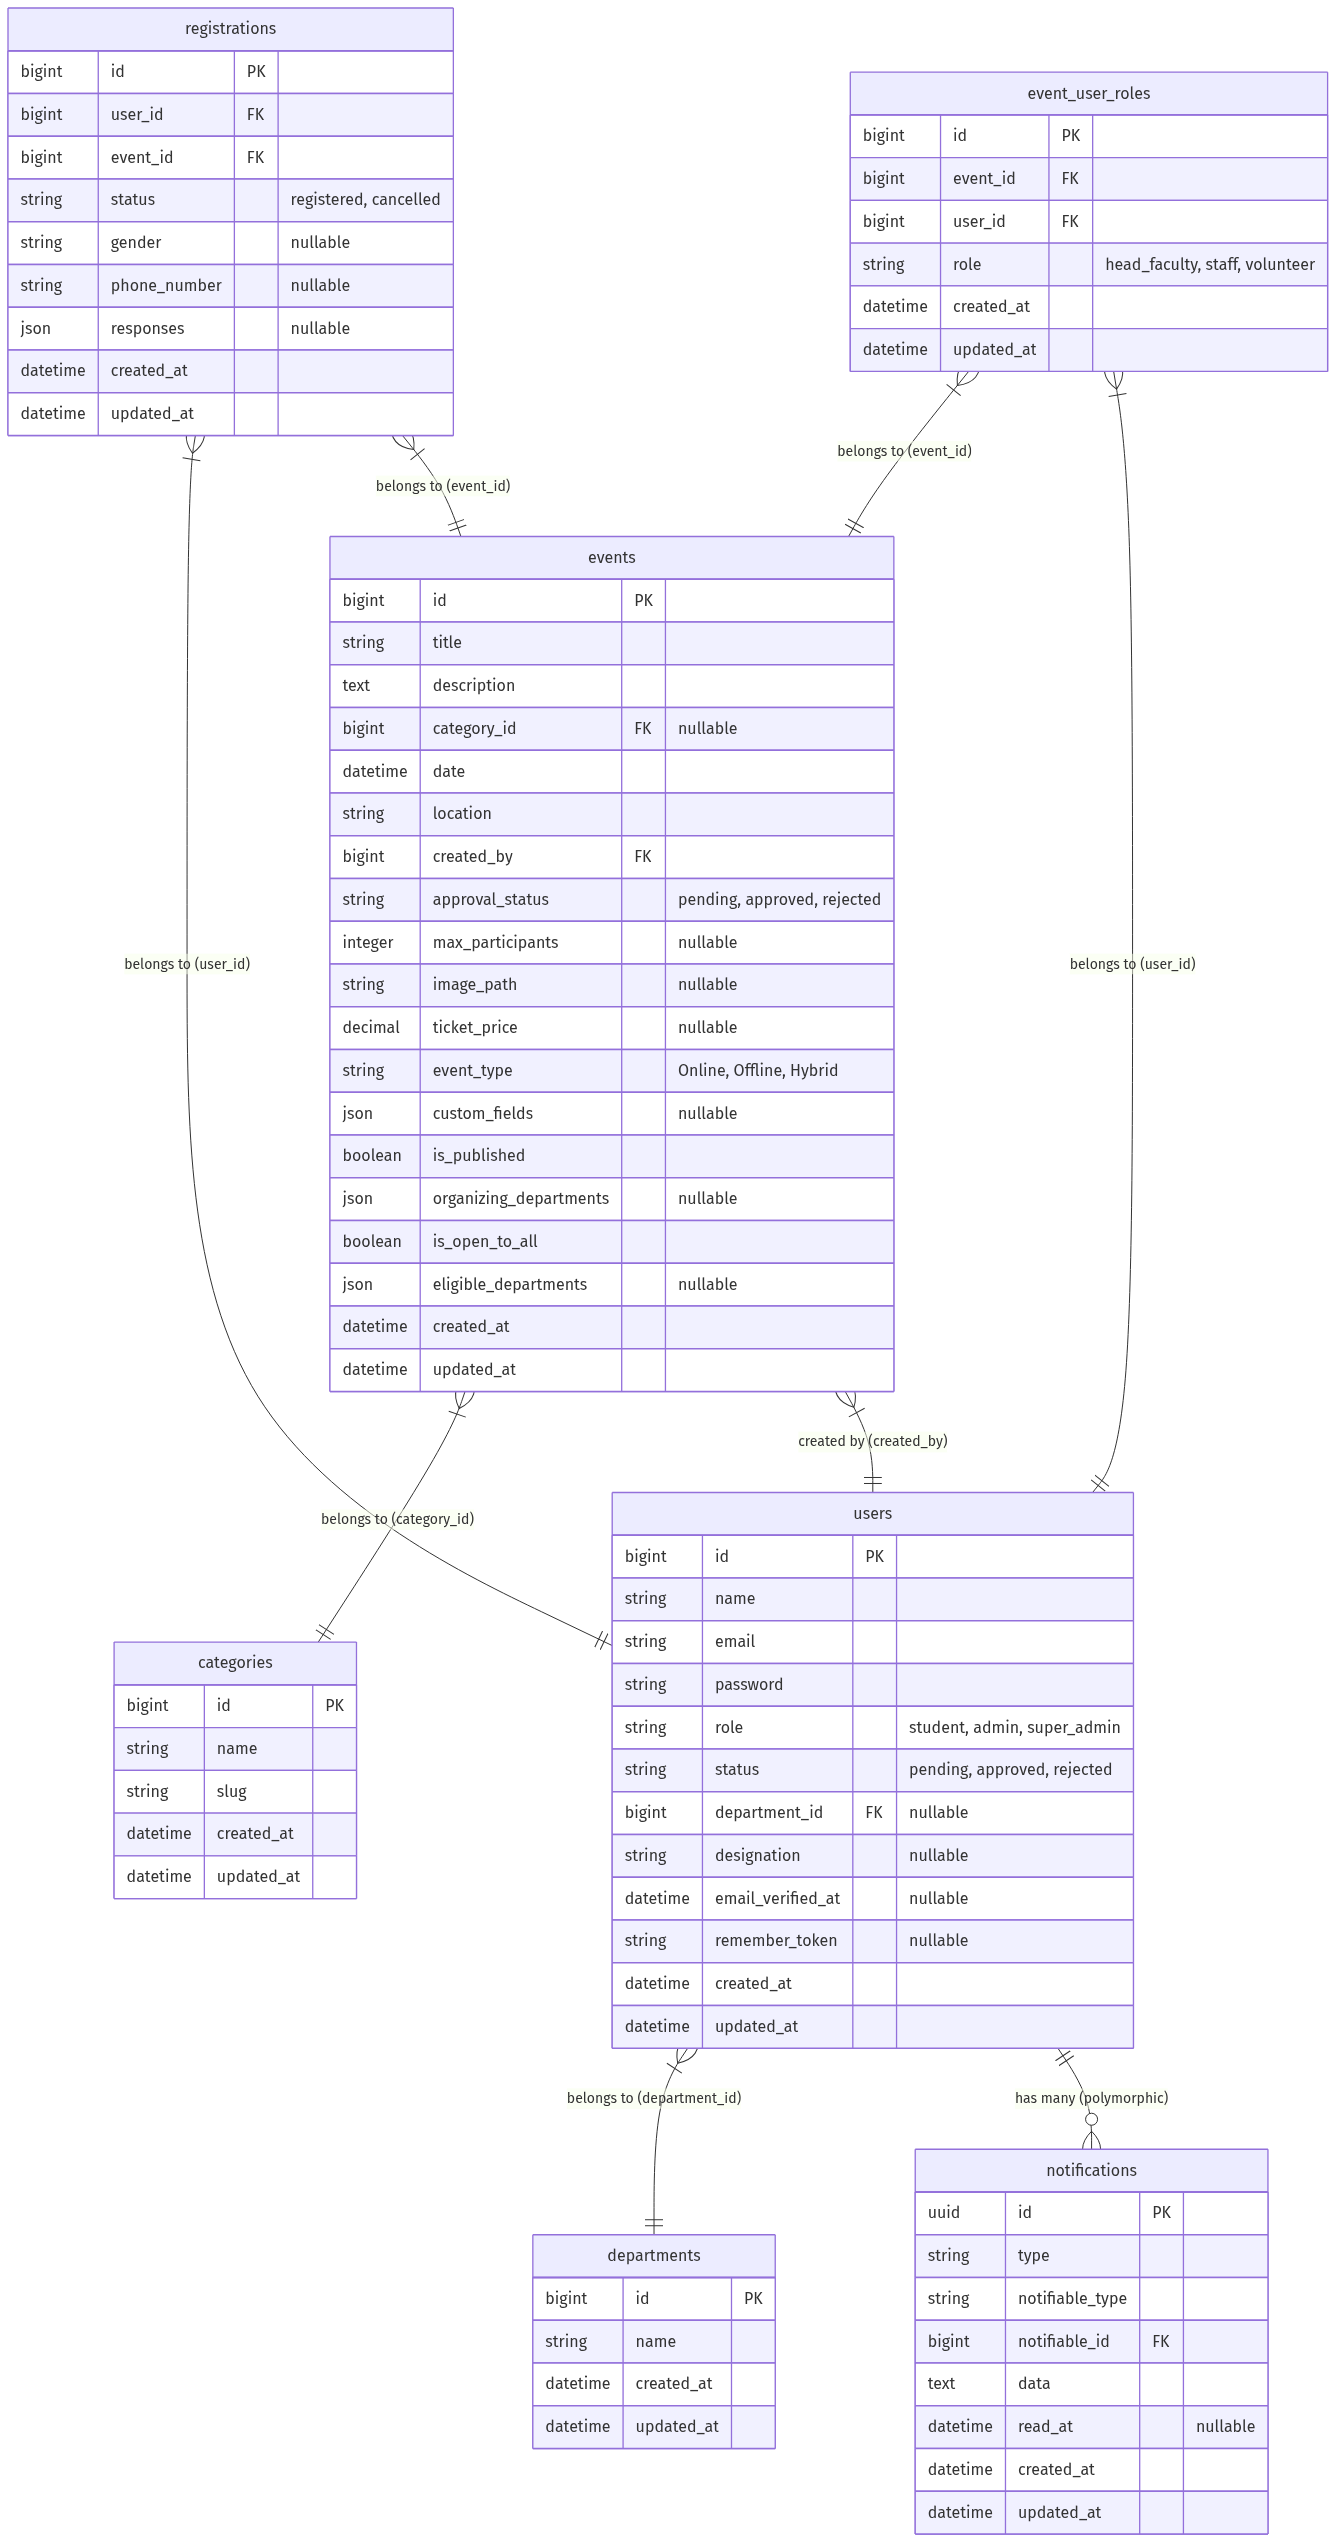
\includegraphics[width=1\textwidth]{erdiagram.png}
    \caption{Entity-Relationship (ER) Diagram}
    \label{fig:er_diagram}
\end{figure}
\textbf{Diagram Explanation:}\\
The ER Diagram displays the primary entities: Users, Events, Categories, Departments, and Registrations. It highlights the relationships, such as a User having many Registrations, an Event belonging to a Category, and Event\_User\_Roles acting as a pivot for the structural organizing team.

\begin{lstlisting}[style=csharpstyle]
// Example of the Event Schema structure via Laravel Migration format
Schema::create('events', function (Blueprint $table) {
    $table->id();
    $table->foreignId('user_id')->constrained()->onDelete('cascade'); // Creator
    $table->string('title');
    $table->text('description');
    $table->dateTime('event_date');
    $table->string('location');
    $table->integer('max_participants');
    $table->string('approval_status')->default('pending'); 
    $table->timestamps();
});
\end{lstlisting}
